\documentclass[12pt,a4paper]{article}

\usepackage[margin=1in]{geometry}
\usepackage{graphicx}
\usepackage{amsmath}
\usepackage{booktabs}
\usepackage{float}
\usepackage{array}
\usepackage{longtable}
\usepackage{setspace}
\usepackage{hyperref}
\usepackage{titlesec}

\setstretch{1.15}
\setlength{\parskip}{0.5em}
\setlength{\parindent}{0pt}
\hypersetup{colorlinks=true,linkcolor=black,urlcolor=blue,citecolor=black}

\titleformat{\section}{\large\bfseries}{\thesection.}{0.5em}{}
\titleformat{\subsection}{\normalsize\bfseries}{\thesubsection}{0.5em}{}

\begin{document}

\begin{titlepage}
\centering

{\Large \textbf{Simulation-Based Implementation of Lean Manufacturing Techniques for Productivity Improvement in SMEs:}}\\[0.3cm]
{\Large \textbf{A Data-Driven Case Study From a Beverage Bottling Line}}\\[1.2cm]

{\large \textbf{Final Research Paper}}\\[1cm]

\begin{tabular}{>{\bfseries}p{4.2cm}p{9.5cm}}
Submitted by & Divash Krishnam, Ashutosh Verma, Raja \\
  \\
Department & Production and Industrial Engineering \\
Guided by & Dr.\ MOHD SHUAIB \\
Guide Department & Mechanical Department \\
\end{tabular}

\vfill

{\large Department of Production and Industrial Engineering}\\[0.2cm]
{\large Under the Guidance of Dr.\ MOHD SHUAIB, Mechanical Department}\\[0.8cm]
{\large \today}

\end{titlepage}

\tableofcontents
\newpage

\section*{Abstract}
The paper shows result how lean manufacturing methods can be priorities in an SME beverage bottling line using real production and downtime records. The dataset has 59 production summaries, 265 hourly observations, and 1,388 downtime events recorded from July 22, 2022, to February 6, 2023. A bootstrap simulation with 5,000 replications tested three lean scenarios: 5S with visual management, TPM, and an integrated lean bundle. The factory's production line produced 212,358 liters, but only 42.66\% of observed time was value-adding; the rest of 57.64\% was consumed by waiting and waste. Micro-stoppages accounted for 61.31\% of all events but only 13.59\% of downtime minutes, whereas major stoppages accounted for 6.77\% of events yet consumed 66.26\% of lost time. 5S improved output by 2.33\%; TPM improved output by 20.61\%; the integrated bundle improved output by 32.19\% and raised availability from 42.37\% to 55.33\%. The key finding is that the most impactful first action targets the most costly stoppage, not the most visible one.

\section*{Keywords}
Lean manufacturing, productivity improvement, SME manufacturing, waste reduction, waiting waste, beverage bottling line, downtime analysis, total productive maintenance, 5S, bootstrap simulation.

\newpage
\section{Introduction}
\subsection{Background and Motivation}
Manufacturing remains a critical driver of economic output and employment, particularly in developing economies where small and medium-sized enterprises (SMEs) form the backbone of industrial activity. Despite their numerical significance, SMEs consistently operate below their productive potential, constrained by limited maintenance capacity, restricted improvement budgets, and the absence of structured operational frameworks [1]. Lean manufacturing, originally developed within large-scale automotive environments, offers a rigorous set of tools for identifying and eliminating production waste. However, as Belhadi et al. [18] demonstrate, the adoption of lean methods in SMEs is shaped by resource constraints, sequencing difficulties, and measurement challenges that distinguish them from the large-firm contexts in which most lean knowledge has been generated. This gap is particularly evident in the food and beverage sector, where Dora et al. [19] found that lean practices among European food-processing SMEs remain immature and heavily dependent on internal expertise and workforce capability.

A recurring challenge in SME lean adoption is the absence of a data-driven method for selecting which lean intervention to prioritize first. Most existing studies confirm that lean tools improve performance in general terms, but few translate observed plant-level loss patterns into an explicit, reproducible prioritization framework [3]--[5]. In repetitive production environments such as beverage bottling lines, downtime is the dominant source of waiting waste---monitored time during which the line is idle and no output is generated. Yet, as Zennaro et al. [21] and Inyiama and Oke [22] show, the structure of downtime is rarely uniform: infrequent but severe stoppages can consume a disproportionately large share of lost time, while frequent micro-stoppages may appear disruptive without contributing significantly to total downtime minutes. Failing to distinguish between these categories can easily lead to misdirected improvement efforts, particularly when maintenance and operational resources are already limited.

This study is motivated by the need for a practical, open-data approach that connects observed downtime structure to lean intervention selection in an SME bottling context. The analysis draws on a real IIoT-monitored industrial dataset published by David et al. [7], [8], comprising 1,388 downtime events and 265 hourly operating records collected across a seven-month production horizon. Rather than relying on theoretical frameworks or proprietary case data, this paper applies an event-level bootstrap simulation with 5,000 replications to test three lean scenarios---5S with visual management, Total Productive Maintenance (TPM), and an integrated lean bundle---and evaluates each against throughput recovery, availability improvement, and waiting-waste reduction. The goal is to provide SME managers and researchers with a reproducible, loss-driven method for determining which lean action delivers the highest operational return given the specific stoppage structure of their production system.

\subsection{Problem Statement and Study Objectives}
Not every problem on a bottling line costs the same amount of time. A typical plant may see dozens of short stoppages or interruptions during a shift, but only a few longer stoppages can consume most of the available production time. In lean manufacturing we call this waiting waste (monitored time passes, but no output is produced). For SMEs, this makes prioritization difficult because maintenance capacity, technical manpower, and improvement budgets are usually limited [1], [3].

In practice, the first improvement decision in a plant is often the hardest one because it can cause productivity loss if the step taken is not good. Managers may know that downtime is hurting output, but they are still uncertain whether to focus on workplace discipline, maintenance, line organization, or some combination of these actions. A useful research study should show that they need to do more than describe lean tools in general terms. It should show which loss is more in the observed system and estimate what level of improvement they can follow to reduce that loss.

This paper shows the above problem through a real beverage bottling dataset collected from an IIoT-enabled production system [7], [8]. Because the dataset contains all the input required for the lean action, it can connect directly to observed operating losses and estimate how much waiting waste each method can remove. Instead of treating lean manufacturing only as a theoretical framework, this paper uses plant data to test which method is most likely to recover productive time and reduce wasting time.

The purpose of the study is to develop a clear, data-based method for selecting lean methods in a repetitive production environment. The same approach is also useful as an academic case because it combines industrial-engineering analysis, production data, and simulation in a form that can be checked against actual operating records rather than only theoretical claims.

The main objectives of this study are:
\begin{enumerate}
    \item to analyze the production behavior and downtime structure of a real bottling-line system;
    \item to identify the dominant waiting-waste pattern affecting productivity;
    \item to simulate the effect of selected lean interventions on throughput, availability, and waste reduction; and
    \item to recommend an implementation priority for lean techniques based on the observed loss pattern.
\end{enumerate}

\section{Literature Review}
The literature relevant to this study can be organized into four linked conversations, each showing a different situation of the problem. The first focuses on the general relationship between lean manufacturing and operational performance. Belekoukias et al. [1] study found that lean methods are often linked with improvements in manufacturing performance, but their result depends heavily on context. Belhadi et al. [18], from examining SME contexts, reached a conclusion: lean methods adoption in SMEs is shaped by resource constraints, sequencing problems, and measurement difficulties. By reading together, these studies show lean implementation, but they also indicate that SMEs need help in deciding which methods should come first instead of adopting lean tools randomly without any prior knowledge.

A second study focuses on food and beverage production, where factors like packaging synchronization, hygiene requirements, short stoppages, and high line interdependence make it difficult to directly transfer lean lessons from other industries. Dora et al. [19] found that lean methods used for practicing in European food-processing SMEs were still immature and strongly influenced by workforce capability and internal expertise. Cuggia Jimenez et al. [23] similarly, their review showed that in the food industry, lean research is wide in topic coverage but uneven in method and sector requirement. Matindana and Shoshiwa [9] extend the SME discussion by showing that lean methods practices are associated with better outcomes in food and beverage SMEs, but the research showed it was more practical for the sector level, not for the plant level. These combined studies confirm the importance of lean practices in the food sector, yet they do not guide whether a bottling line should first solve the micro-stoppages, major breakdowns, or both.

A third study is focused on a simulation and model-based evaluation of lean alternatives. Oleghe and Salonitis [2] demonstrate that lean analysis improves when human behavior, process variability, and system interaction are directly monitored or captured instead of being discussed only in theoretical terms. Yu and Chen [3] reached a similar conclusion from an SME perspective: simulation is an important part for improvement planning, but many smaller firms still lack practical and adaptable lean tools that fit their operating reality. Possik et al. [4] also used simulation to compare lean methods under changing manufacturing conditions, while Frecassetti et al.'s [5] results showed that simulation can improve lean-practice selection for an SME before any physical practical implementation starts. Al-Hawari et al. [20] are directly relevant to the present work because their study shows that they used simulation to study productivity improvement in a bottle-filling system and connected downtime analysis to throughput gains. Compared with these studies, the current paper is focused on a smaller set of KPIs, but it is more directly linked to the observed downtime types, specific lean scenarios, and maintaining the workflow replicable with publicly open data.

A fourth study is more directly downtime centered and therefore closer to the core logic of this present study. Zennaro et al. [21] collected the details of micro-downtime data from bottling lines and then showed that short breaks or stoppages represent a large share of inefficiency once they are recorded carefully. Inyiama and Oke [22] examined downtime in a process bottling plant through cause-and-effect analysis, Pareto reasoning, and Weibull modeling. Their findings highlight how maintenance-oriented diagnosis can improve reliability planning. Bokhorst et al. [6] found that smart manufacturing practices tend to build on lean principles rather than replace them, while Reslan et al. [10] applied digital-twin-based value-stream mapping to show how real-time data can strengthen process analysis. These above studies show that the data collected from a specific production line can make lean analysis more precise, particularly when waiting waste must be identified from actual operating behavior rather than observation alone.

\begin{longtable}{p{2.8cm}p{5.7cm}p{4.9cm}}
\caption{Literature Synthesis and Comparative Relevance}\\
\toprule
\textbf{Study} & \textbf{Main Contribution} & \textbf{Gap Relevant to This Study} \\
\midrule
\endfirsthead
\toprule
\textbf{Study} & \textbf{Main Contribution} & \textbf{Gap Relevant to This Study} \\
\midrule
\endhead
Womack and Jones [24] & Defines lean thinking around value, value stream, flow, pull, and continuous waste removal. & Provides the conceptual basis for waste reduction, but does not give a plant-data method for selecting among 5S, TPM, or combined interventions. \\
Shah and Ward [25] & Shows lean production as a bundle of interrelated practices rather than a single isolated tool. & Supports integrated lean thinking, but does not identify which tool should be applied first when stoppage losses are unequal. \\
Bhamu and Sangwan [26] & Reviews lean definitions, tools, indicators, and research issues across a wide body of lean literature. & Strong for broad theory, but limited in event-level downtime prioritization for small production systems. \\
Belhadi \emph{et al.} [18] & Broad review of lean production in SMEs and their implementation challenges. & Strong on SME context, but not designed for plant-level prioritization of specific downtime losses. \\
Dora \emph{et al.} [19] & Connects lean practice to operational performance and critical success factors in food-processing SMEs. & Valuable sector relevance, but limited guidance on event-level stoppage prioritization. \\
Melton [27] & Explains how lean thinking can be adapted to process-industry environments. & Supports the relevance of lean in flow-oriented industries, but does not develop a bottling-line simulation model. \\
Yu and Chen [3] & Review of factory simulation in SMEs and identification of adoption barriers. & Supports simulation use, but does not provide a bottling-line loss-ranking workflow. \\
Possik \emph{et al.} [4] & Co-simulation framework for evaluating lean technique impact under changing conditions. & Broader contextual modeling, but limited open-data reproducibility. \\
Frecassetti \emph{et al.} [5] & Simulation-based introduction of lean practices in an SME. & Helpful for tool selection, but industrial data are not openly reusable. \\
Muchiri and Pintelon [29] & Reviews OEE as a performance-measurement tool linking availability, performance, and quality losses. & Useful for KPI logic, but OEE alone may hide whether downtime is driven by frequent short stops or rare long failures. \\
Dal \emph{et al.} [30] & Shows OEE as a practical measure for directing operational improvement. & Demonstrates improvement measurement, but not a comparative lean-priority framework for bottling-line stoppage categories. \\
Ng Corrales \emph{et al.} [31] & Reviews OEE evolution and its use across different decision-support contexts. & Shows broad OEE adaptability, but not specific SME beverage-line intervention ranking. \\
Zennaro \emph{et al.} [21] & Detailed micro-downtime analysis in beverage bottling lines with OEE relevance. & Strong downtime diagnosis, but not framed as lean-intervention prioritization under uncertainty. \\
Inyiama and Oke [22] & Reliability and downtime evaluation in a process bottling plant using cause-effect and Weibull analysis. & Strong maintenance insight, but not a comparative lean-scenario framework. \\
Ahuja and Khamba [32] & Reviews TPM implementation, enablers, barriers, and success factors. & Supports the maintenance logic behind major-stoppage reduction, but does not quantify bottling-line scenario outcomes with open data. \\
Abdulmalek and Rajgopal [33] & Combines value-stream mapping and simulation to quantify lean benefits in a process-sector case. & Strong simulation relevance, but not focused on SME beverage-line downtime classification. \\
This study & Open-data, downtime-driven simulation of lean alternatives in an SME bottling context. & Focuses on a reproducible case that connects stoppage structure to lean-priority selection. \\
\bottomrule
\end{longtable}

\section{Research Gap and Research Questions}
The review above points to a specific gap. Despite growing evidence that lean practices improve performance, limited research demonstrates how actual breakdown records can be used to choose between competing lean interventions in an SME-relevant production setting [3]--[5], [9], [18], [19]. Most studies confirm that lean works, but few go as far as translating downtime data into an explicit, reproducible measure of waiting-waste reduction.

A second gap concerns data openness. Much of the bottling-line literature relies on proprietary industrial datasets, which makes it difficult for students or smaller firms to replicate the same analytical steps using publicly accessible data [20]--[22].

A third gap concerns methodological fit. Not all existing approaches are equally suited to repetitive packaging systems, where stoppage severity directly determines the extent of output loss and waiting waste. Few methods are specifically designed around this relationship.

To address that gap, the present study is guided by the following research questions:
\begin{enumerate}
    \item Which stoppage type causes the most damage to productivity?
    \item How much does each lean strategy actually improve things when tested?
    \item Given unequal stoppage impact, which lean action should come first?
\end{enumerate}

\section{Research Objective}
The focus of this study is a real beverage bottling line, represented through a publicly available dataset published on Zenodo in January 2026 [8]. Unlike studies that are based on simulated or proprietary data, this research draws on an openly accessible industrial dataset collected from a real IIoT-monitored bottling operation, and the related article by David et al. [7] confirms the industrial and digital-monitoring context of the source.

The dataset consists of four groups of information:
\begin{enumerate}
    \item hourly production output records,
    \item daily production summaries,
    \item hourly operating breakdown records, and
    \item individual breakdown event records.
\end{enumerate}

The monitoring period spans approximately seven months, from July 2022 to February 2023. The inclusion of two product sizes, 3-liter and 5-liter containers, captures real-time changes in line behavior over the time period. What makes this dataset particularly suitable is that it captures both production performance and detailed stoppage events, which makes it suitable for a study focused on lean prioritization through observed loss patterns.

\begin{table}[H]
\centering
\caption{Dataset Characteristics}
\begin{tabular}{lr}
\toprule
\textbf{Attribute} & \textbf{Value} \\
\midrule
Monitoring period & July 22, 2022 to February 6, 2023 \\
Production summary records & 59 \\
Calendar production days & 56 \\
Hourly operating observations & 265 \\
Downtime events & 1,388 \\
Observed product sizes & 3 L and 5 L \\
Total liters produced & 212,358 \\
Total units produced & 60,888 \\
Total monitored time & 238.65 h \\
Total operating time & 101.81 h \\
\bottomrule
\end{tabular}
\end{table}

\section{Methodology}
This paper uses a data-driven simulation methodology to find out lean alternatives on the basis of observed production behavior. The method combines baseline performance analysis, downtime classification, waiting-waste measurement, and bootstrap simulation.

\subsection{Analytical Framework}
\begin{equation}
A = \frac{T_{op}}{T_{mon}}
\end{equation}
where $A$ is operational availability, $T_{op}$ is effective operating time, and $T_{mon}$ is monitored time.

\begin{equation}
T_{dt} = T_{mon} - T_{op}
\end{equation}
where $T_{dt}$ is downtime or pause time.

\begin{equation}
R = \frac{Q}{T_{op}}
\end{equation}
where $Q$ is total production output in liters and $R$ is the average production rate in liters per operating hour.

\begin{equation}
Q' = R \times (T_{mon} - T'_{dt})
\end{equation}
where $Q'$ is the simulated output after a lean intervention and $T'_{dt}$ is the scenario-adjusted downtime.

\begin{equation}
T'_{dt} = T_{res} + \sum_{i=1}^{n}\alpha_i t_i
\end{equation}
where $T_{res}$ is residual downtime not explicitly represented at event level, $t_i$ is the duration of downtime event $i$, and $\alpha_i$ is a scenario-specific reduction factor applied to that event.

\begin{equation}
\%\Delta Q = \frac{Q' - Q}{Q}\times 100
\end{equation}

\begin{equation}
\%\Delta W = \frac{T_{dt} - T'_{dt}}{T_{dt}}\times 100
\end{equation}
where $\%\Delta W$ is the percentage reduction in waiting waste after a lean intervention.

These relationships were used to convert plant observations into comparable scenario outcomes for throughput, availability, and waste reduction.

\subsection{Step 1: Data Extraction and Cleaning}
The Excel dataset [8] was organized into production summaries, hourly operation records, and downtime-event data. Dates, durations, and production quantities were standardized. Downtime durations were converted to minutes so that event-level categorization and simulation could be performed consistently.

\subsection{Step 2: Baseline Performance Analysis}
Baseline performance was measured using liters produced, production units, monitored time, operating time, pause time, daily efficiency, hourly efficiency, and the share of monitored time consumed by waiting waste. This step was necessary to understand the real operating condition of the system before any lean scenario was introduced.

\subsection{Step 3: Downtime Categorization}
Downtime events were classified into three categories:
\begin{itemize}
    \item \textbf{Micro-stoppages:} $t \leq 2$ min
    \item \textbf{Minor stoppages:} $2 < t \leq 10$ min
    \item \textbf{Major stoppages:} $t > 10$ min
\end{itemize}

This classification distinguishes frequent short interruptions from serious breakdown-type events. Such separation is important for selecting lean tools.

\subsection{Step 4: Production-Rate Estimation}
For each observed production day, production rate was estimated from liters produced divided by effective operating time. This creates a realistic day-level performance profile that preserves operational variability instead of assuming a constant theoretical output rate.

\subsection{Step 5: Bootstrap Simulation}
This study applies an event-level bootstrap simulation with 5,000 replications. Each replication resampled observed day profiles with replacement. This action preserves the stochastic behavior of monitored time, productivity, and downtime structure. Event durations were normalized to the recorded daily pause time so that the simulated baseline consistently reflected the observed plant record.

Bootstrap simulation was selected because it preserves the variability observed in the plant data without assuming any mathematical pattern such as a normal or exponential distribution [17].

\subsection{Step 6: Scenario Design}
The study evaluated three lean scenarios:
\begin{enumerate}
    \item \textbf{5S + Visual Management:} 15\% of micro-stoppages eliminated [12], [13].
    \item \textbf{TPM:} 25\% reduction in the duration of major stoppages [14], [15].
    \item \textbf{Integrated Lean Bundle:} 20\% of micro-stoppages eliminated, 15\% reduction in minor stoppages, and 30\% reduction in major stoppages [16].
\end{enumerate}

These values above are informed by lean implementation logic and literature [12]--[16]. They are intended for final comparison rather than claiming exact future plant outcomes.

The scenario values were not chosen randomly. The 5S assumption was based on reported 5S case improvements such as 8--18\% reductions in operational time and substantial efficiency gains in SME [12], [13]. The TPM assumption was based on TPM case studies reporting about 23--23.4\% reductions in breakdowns or downtime, with more reduction of downtime in some specific industries [14], [15]. The integrated lean bundle combines these tools' effects and follows the wider evidence that the integrated bundle will give more operational results than a single or isolated tool [16]. For that reason, the scenario values should be read as literature-grounded planning parameters rather than randomly hypothetical numbers or exact guarantees of future plant outcomes.

\subsection{Algorithmic Logic of the Proposed Model}
The model uses a data-driven bootstrap simulation. First, daily production and downtime records are converted into baseline operating profiles. Second, these observed day profiles are resampled with replacement across 5,000 replications to preserve real production variability. Third, lean rules are applied to the sampled downtime events. Finally, pause time, operating time, availability, output, and waiting-waste reduction are recalculated.

In operational terms, the algorithm does not impose an artificial production pattern on the system. It repeatedly resamples the behavior observed in the real plant and then estimates how the results change when specific categories of downtime are reduced through lean interventions.

\subsection{How Lean Manufacturing Was Applied to the Data}
Lean manufacturing was applied directly to the downtime data by mapping each lean tool to a loss category specifically. In this paper, downtime is calculated as waiting waste because observed production time is used without generating output.

\begin{table}[H]
\centering
\caption{How Lean Tools Were Mapped to the Data}
\begin{tabular}{p{3.0cm}p{4.2cm}p{6.0cm}}
\toprule
\textbf{Lean Tool} & \textbf{Data Signal Used} & \textbf{Logic Used in the Model} \\
\midrule
5S + Visual Management & Micro-stoppages and short interruptions & Better workplace organization is expected to remove small avoidable delays and short flow interruptions. \\
TPM & Major stoppages and long downtime duration & Better maintenance and reliability are expected to reduce severe breakdown time and recovery time. \\
Integrated Lean Bundle & Micro, minor, and major stoppages together & A combined lean program is expected to improve both routine discipline and machine reliability. \\
\bottomrule
\end{tabular}
\end{table}

\section{Result}
\subsection{Baseline Performance of the System}
The recorded production system produced 212,358 liters from 60,888 units during 238.65 monitored hours. However, the operating time was only 101.81 hours, while pause time reached 137.56 hours. This shows an overall observed availability of 42.66\%, showing that downtime is the main dominant constraint. The same result can be read in lean terms: waiting waste was 57.64\% of monitored time, with the remaining 42.66\% as the total observed time during which the real production happened.

While looking at each product separately, the average production rate was 1,963.71 L/h for the 3-liter product and 2,918.68 L/h for the 5-liter product. Therefore, the 5-liter product showed a higher effective throughput during operating time.

\begin{table}[H]
\centering
\caption{Baseline Performance Indicators}
\begin{tabular}{lr}
\toprule
\textbf{Metric} & \textbf{Value} \\
\midrule
Production days & 56 \\
Production summary records & 59 \\
Hourly observations & 265 \\
Downtime events & 1,388 \\
Total production & 212,358 L \\
Total units produced & 60,888 \\
Monitored time & 238.65 h \\
Operating time & 101.81 h \\
Pause time & 137.56 h \\
Overall availability & 42.66\% \\
Waiting-waste share & 57.64\% \\
Value-adding time share & 42.66\% \\
\bottomrule
\end{tabular}
\end{table}

\begin{figure}[H]
\centering
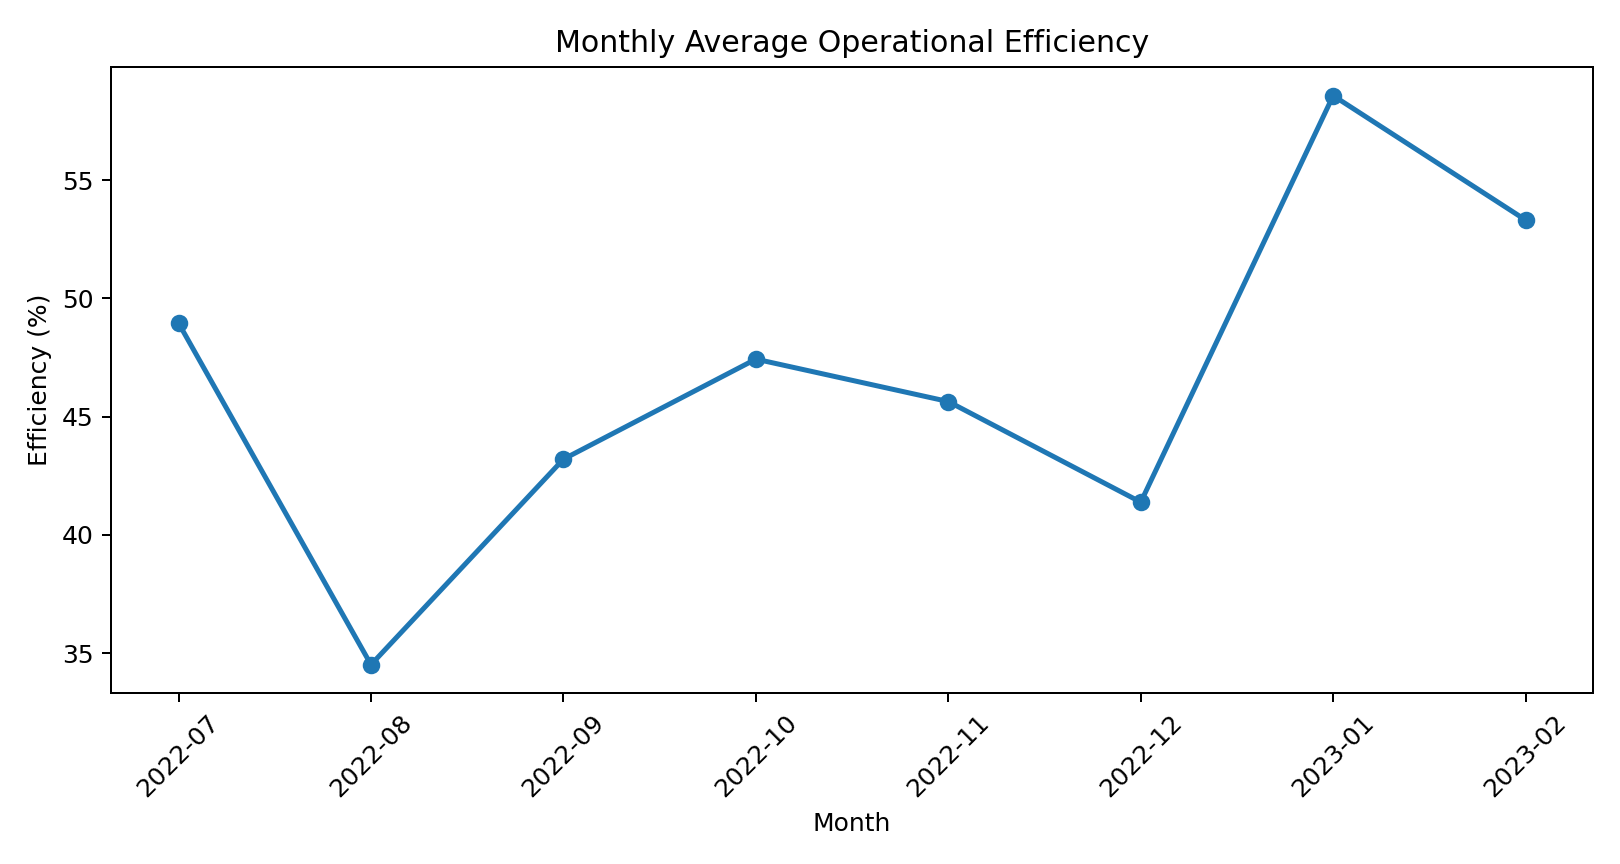
\includegraphics[width=0.92\textwidth]{outputs/monthly_efficiency.png}
\caption{Monthly average operational efficiency from the real bottling-line dataset.}
\end{figure}

The monthly efficiency chart shows different variations across the study period. Lower performance is seen in August 2022 and December 2022, while stronger operational performance was seen in January 2023. This confirms that the production line does not behave like a stable production system.

\subsection{Downtime Structure}
The downtime-event distribution is heavily on the left side, where the timing of the stoppages was less than 2 minutes. The median event duration is 1.50 minutes; 90\% of all the events fall below 6.50 minutes; the 95th percentile reaches 13.74 minutes; and the longest recorded event is 349.83 minutes. These statistics confirm that the production line experiences many short interruptions but also a small number of very large disruptions.

\begin{figure}[H]
\centering
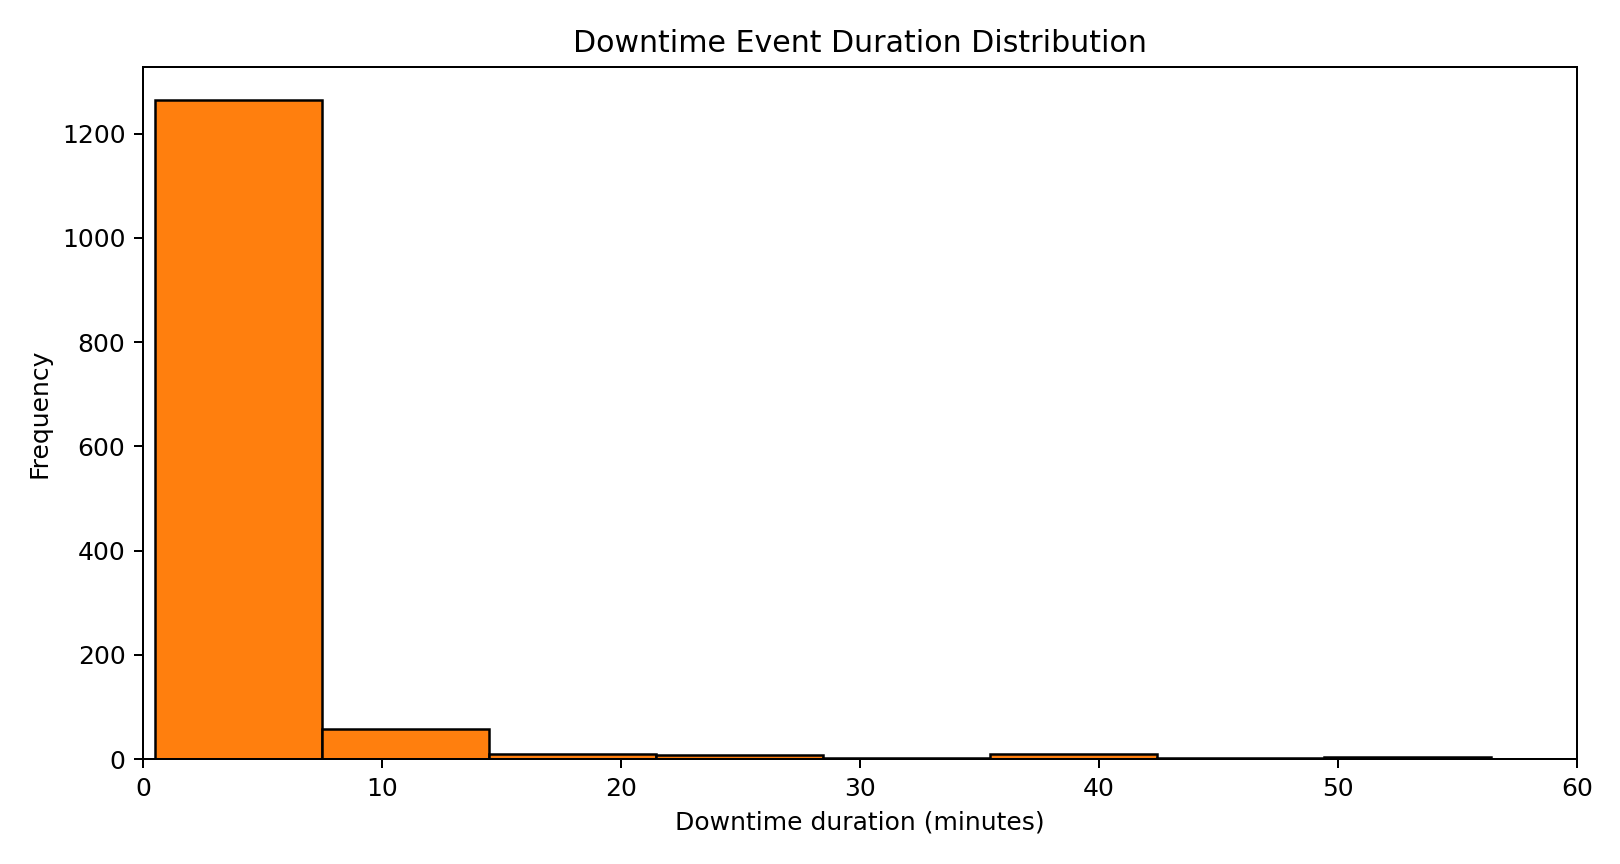
\includegraphics[width=0.92\textwidth]{outputs/downtime_distribution.png}
\caption{Distribution of downtime-event duration, truncated at 60 minutes for readability.}
\end{figure}

\begin{table}[H]
\centering
\caption{Downtime Category Structure}
\begin{tabular}{lrr}
\toprule
\textbf{Category} & \textbf{Event Count} & \textbf{Share of Downtime Minutes} \\
\midrule
Micro ($\leq$ 2 min) & 851 & 13.59\% \\
Minor (2--10 min) & 443 & 20.15\% \\
Major ($>$ 10 min) & 94 & 66.26\% \\
\bottomrule
\end{tabular}
\end{table}

\begin{figure}[H]
\centering
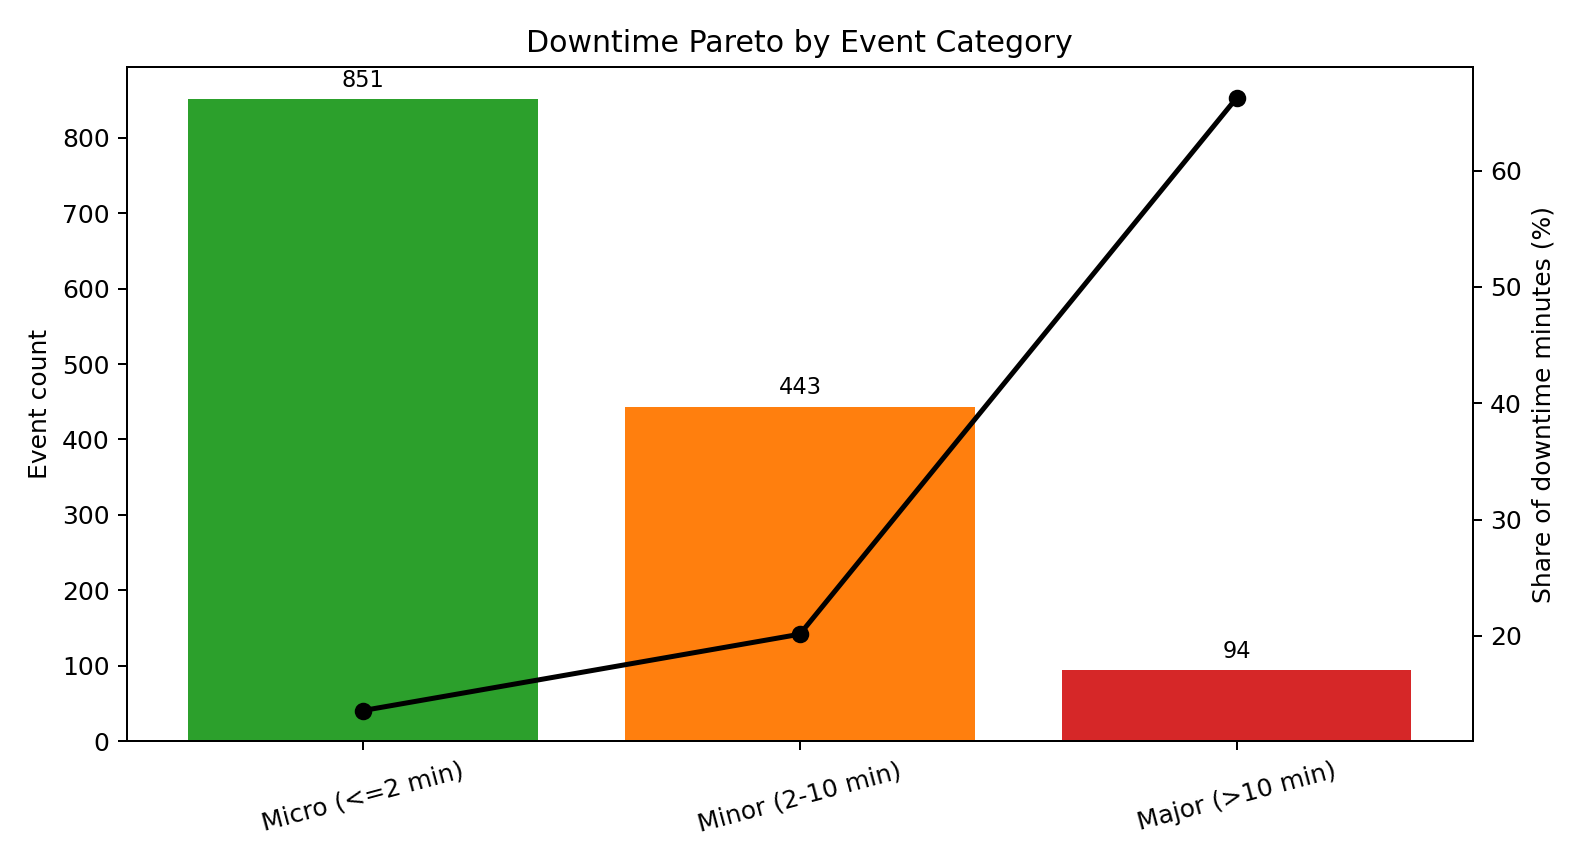
\includegraphics[width=0.92\textwidth]{outputs/downtime_category_pareto.png}
\caption{Downtime Pareto by event category. Major stoppages are rare but dominant in lost time.}
\end{figure}

Micro-stoppages account for 61.31\% of all events but only contribute 13.59\% of total downtime (in minutes), whereas major stoppages represent only 6.77\% of events but consume most of the 66.26\% of lost downtime. This means that the frequency of the events alone cannot identify the highest productivity loss. In real plant conditions, this can easily lead to misdirected improvement efforts.

\subsection{Pause Time and Efficiency Relationship}
When the data is grouped by date, pause time shows that it is inversely proportional to efficiency ($r=-0.707$). This means that as the daily pause time increases, effective production line operating efficiency falls sharply.

\begin{figure}[H]
\centering
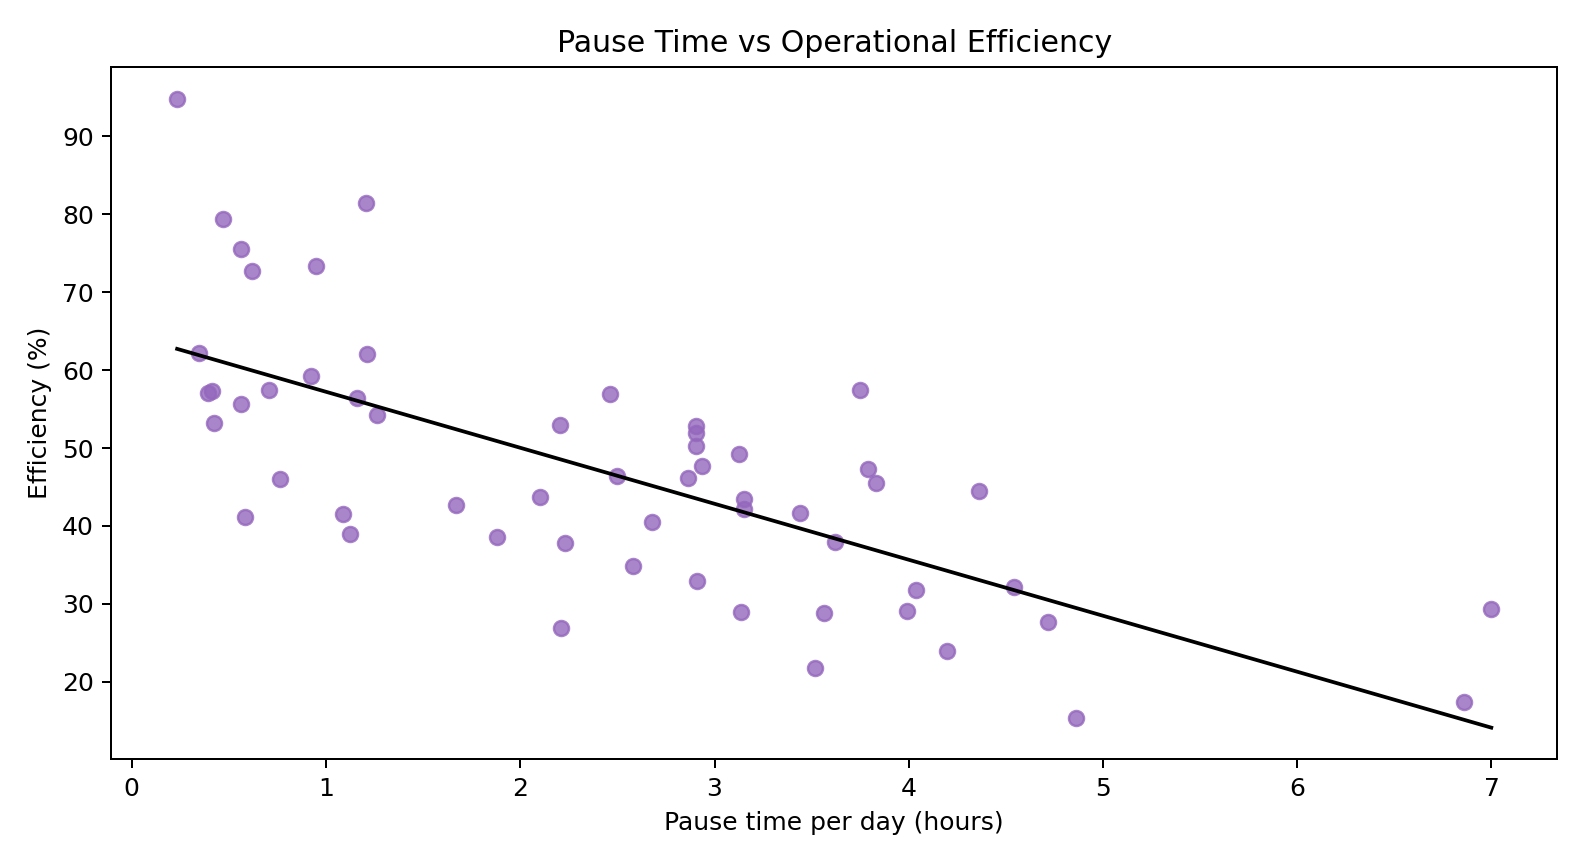
\includegraphics[width=0.92\textwidth]{outputs/pause_vs_efficiency.png}
\caption{Daily pause time versus operational efficiency.}
\end{figure}

\subsection{Production Rate by Product Type}
The production-rate comparison by product size is shown below.

\begin{figure}[H]
\centering
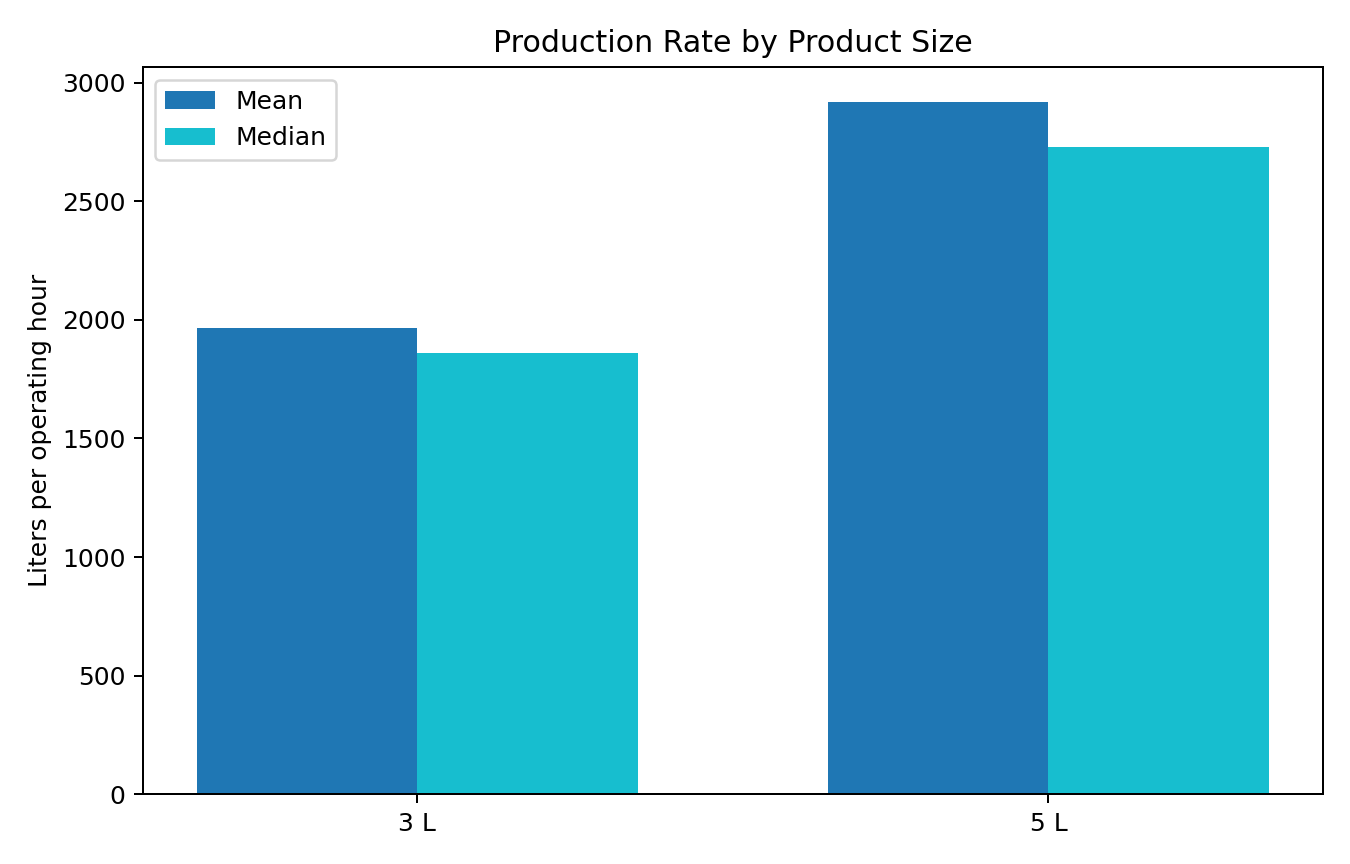
\includegraphics[width=0.85\textwidth]{outputs/product_rate_comparison.png}
\caption{Mean and median production rate by product size.}
\end{figure}

The 5-liter product produced consistently higher production rates than the 3-liter product in both average and median output. This suggests that product mix can also influence line performance.

\subsection{Simulation Results}
The simulation baseline produced 211,924.69 liters, very close to the real system's 212,358 liters. This indicates that the simulation performed was reliable and reflects actual plant behavior. In the baseline simulation, waiting waste averaged 137.67 hours, which represents 57.67\% of monitored time.

\begin{table}[H]
\centering
\caption{Simulation Results for Lean Scenarios}
\begin{tabular}{lrrrr}
\toprule
\textbf{Scenario} & \textbf{Mean Output (L)} & \textbf{Gain (\%)} & \textbf{Efficiency (\%)} & \textbf{Eff. Gain (pp)} \\
\midrule
Baseline & 211,924.69 & 0.00 & 42.37 & 0.00 \\
5S + Visual Management & 216,866.69 & 2.33 & 43.25 & 0.88 \\
TPM & 255,604.10 & 20.61 & 50.81 & 8.44 \\
Integrated Lean Bundle & 280,142.22 & 32.19 & 55.33 & 12.96 \\
\bottomrule
\end{tabular}
\end{table}

\begin{table}[H]
\centering
\caption{Waste-Reduction Results for Lean Scenarios}
\begin{tabular}{lrrr}
\toprule
\textbf{Scenario} & \textbf{Waiting Waste (h)} & \textbf{Waste Recovered (h)} & \textbf{Waste Reduction (\%)} \\
\midrule
Baseline & 137.67 & 0.00 & 0.00 \\
5S + Visual Management & 135.57 & 2.10 & 1.52 \\
TPM & 117.46 & 20.21 & 14.68 \\
Integrated Lean Bundle & 106.68 & 30.99 & 22.51 \\
\bottomrule
\end{tabular}
\end{table}

\begin{table}[H]
\centering
\caption{Simulation Uncertainty Range}
\begin{tabular}{lrr}
\toprule
\textbf{Scenario} & \textbf{P05 Output (L)} & \textbf{P95 Output (L)} \\
\midrule
Baseline & 188,572.81 & 236,799.79 \\
5S + Visual Management & 192,906.87 & 242,100.46 \\
TPM & 226,295.58 & 287,389.24 \\
Integrated Lean Bundle & 247,828.10 & 314,804.33 \\
\bottomrule
\end{tabular}
\end{table}

\begin{figure}[H]
\centering
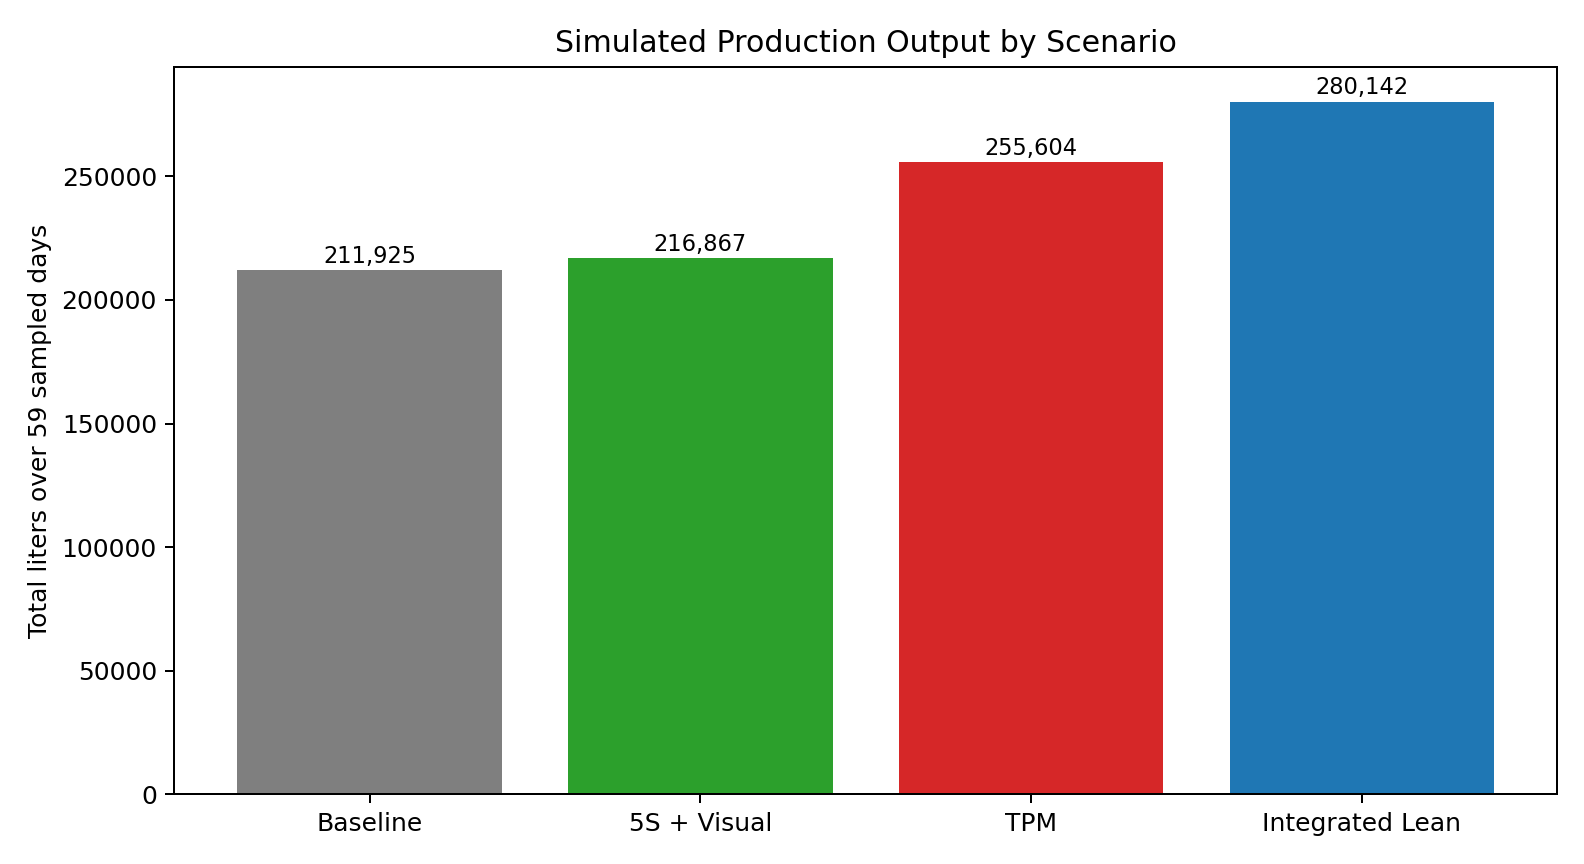
\includegraphics[width=0.92\textwidth]{outputs/scenario_output.png}
\caption{Mean simulated production output across the baseline and lean scenarios.}
\end{figure}

\begin{figure}[H]
\centering
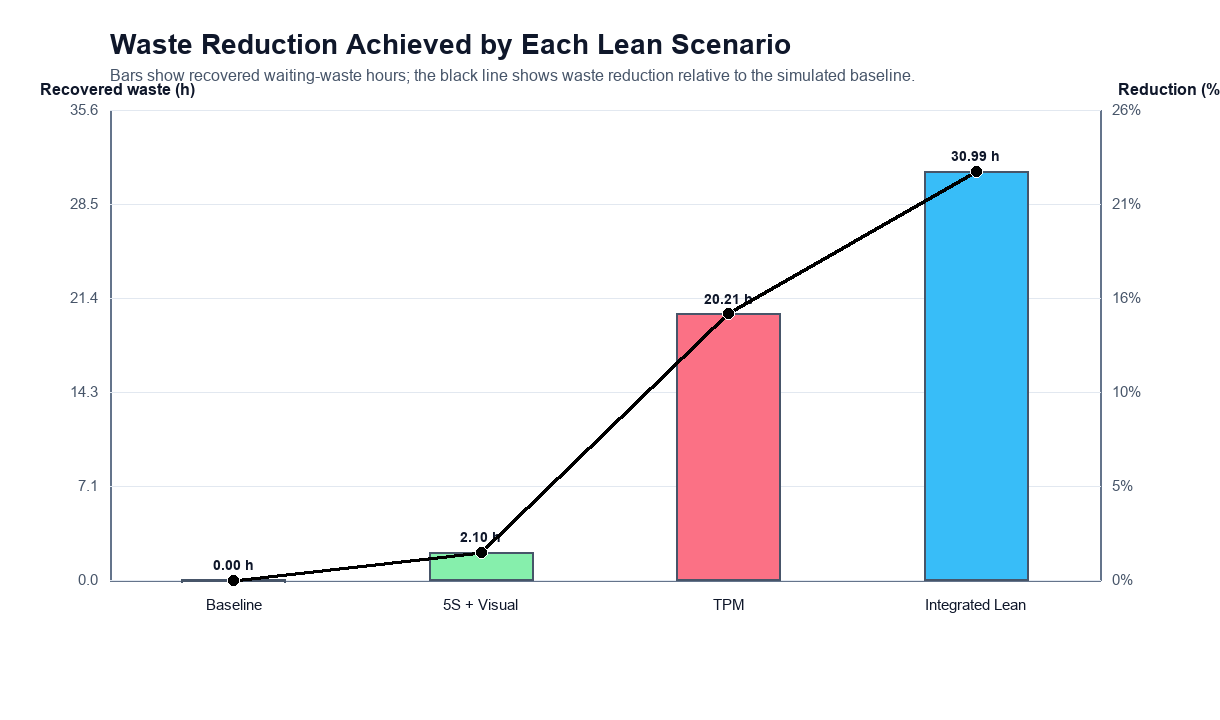
\includegraphics[width=0.94\textwidth]{outputs/scenario_waste_reduction.png}
\caption{Recovered waiting waste and waste-reduction percentage across the simulated lean scenarios.}
\end{figure}

From the simulation, we can see that 5S and visual management provide only a little gain of 2.33\%, which is equivalent to the recovery of 2.10 hours of waiting time. This is because the scenario mainly targets micro-stoppages, which have high frequency but low contribution to the waiting waste. By comparing it with TPM, the TPM produces a much larger gain of 20.61\% and recovers 20.21 hours of waiting waste because it directly targets major stoppages, which have the high margin in the downtime waste. The integrated lean bundle produces the highest gain, improving output by 32.19\%, increasing simulated availability from 42.37\% to 55.33\%, and reducing waiting waste by 22.51\%, which lowers the waiting-waste share from 57.67\% to 44.69\%.

\section{Discussion}
The result tells us that the lean implementation should be based on the structure of loss of operation. Practically, this means that managers may need to reconsider focusing only on frequency interruptions and instead pay close attention to high-impact downtime rather than the visibility or frequency of events alone. In most production systems, micro-stoppages catch the attention because they happen often and interrupt daily work. In the present case, however, the largest production losses and the largest share of waiting waste are connected with major stoppages.

For the bottling line studied here, major stoppages are the real productivity drivers. Although they are comparatively rare, they eat most of the downtime minutes and therefore most of the waiting waste. This shows why TPM, which focuses on equipment reliability and breakdown reduction, produces far more improvement than 5S alone. The result is fully consistent with the broader lean-simulation literature, which emphasizes context-specific tool selection [4], [5].

One more important implication is the role of digital manufacturing data in strengthening lean analysis. Instead of focusing on only static value stream mapping or qualitative observation, this paper uses event-level downtime records and simulation to quantify both output recovery and waste reduction. This is aligned with the direction suggested by smart manufacturing and digital twin research [6], [10].

\subsection{Comparison with Other Methodologies}
The suggested method can also be compared with other lean-evaluation approaches. The comparison used in this paper scores methodologies on Key Performance Index priority, methodological capability, and industry fit. Those scores are interpretive rather than experimental, but they help to locate the present work in the wider range of the literature.

\begin{longtable}{p{2.15cm}p{2.6cm}p{2.45cm}p{3.15cm}p{3.35cm}}
\caption{Methodology Comparison with Related Lean-Evaluation Studies}\\
\toprule
\textbf{Study} & \textbf{Method} & \textbf{Primary KPIs} & \textbf{Strongest Use Case} & \textbf{Main Limitation} \\
\midrule
\endfirsthead
\toprule
\textbf{Study} & \textbf{Method} & \textbf{Primary KPIs} & \textbf{Strongest Use Case} & \textbf{Main Limitation} \\
\midrule
\endhead
This study & Open-data event-level bootstrap simulation & Throughput, availability, downtime, waiting-waste reduction & Repetitive packaging and food-beverage SME lines with downtime logs & Does not directly model quality, WIP, labor, or cost; scenario effects are still assumed rather than observed. \\
Possik \emph{et al.} [4] & Co-simulation for contextual lean-tool evaluation & WIP, lead time, throughput, defect rate & High-mix aerospace and context-sensitive manufacturing systems & Higher modeling burden and weaker accessibility for low-resource SME studies. \\
Frecassetti \emph{et al.} [5] & Mixed case study plus simulation & Process performance and tool-combination impact & Practical SME planning and tool-combination selection & Less event-level downtime specificity in the published description. \\
Oleghe and Salonitis [2] & Hybrid system dynamics and DES & Quality performance, throughput, scheduling trade-off & Plants where workforce behavior and production pressure shape outcomes & Harder to calibrate and less directly usable with simple downtime logs. \\
Reslan \emph{et al.} [10] & Digital twin plus automated VSM & Non-value-added time, resource utilization, process monitoring & Digitally instrumented smart-factory cells & Requires digital-twin infrastructure and higher implementation cost. \\
Matindana and Shoshiwa [9] & Survey-based SEM across SMEs & Output improvement, waste reduction, lean-process adoption & Sector-level benchmarking for food and beverage SMEs & Not suitable for plant-level what-if simulation or downtime-priority analysis. \\
Unal and Bilget [11] & DES plus line-balancing algorithm & Production time, throughput per day, throughput per operator & Labor-intensive assembly and apparel lines & Less informative for automated downtime-dominated packaging systems. \\
\bottomrule
\end{longtable}

\begin{figure}[H]
\centering
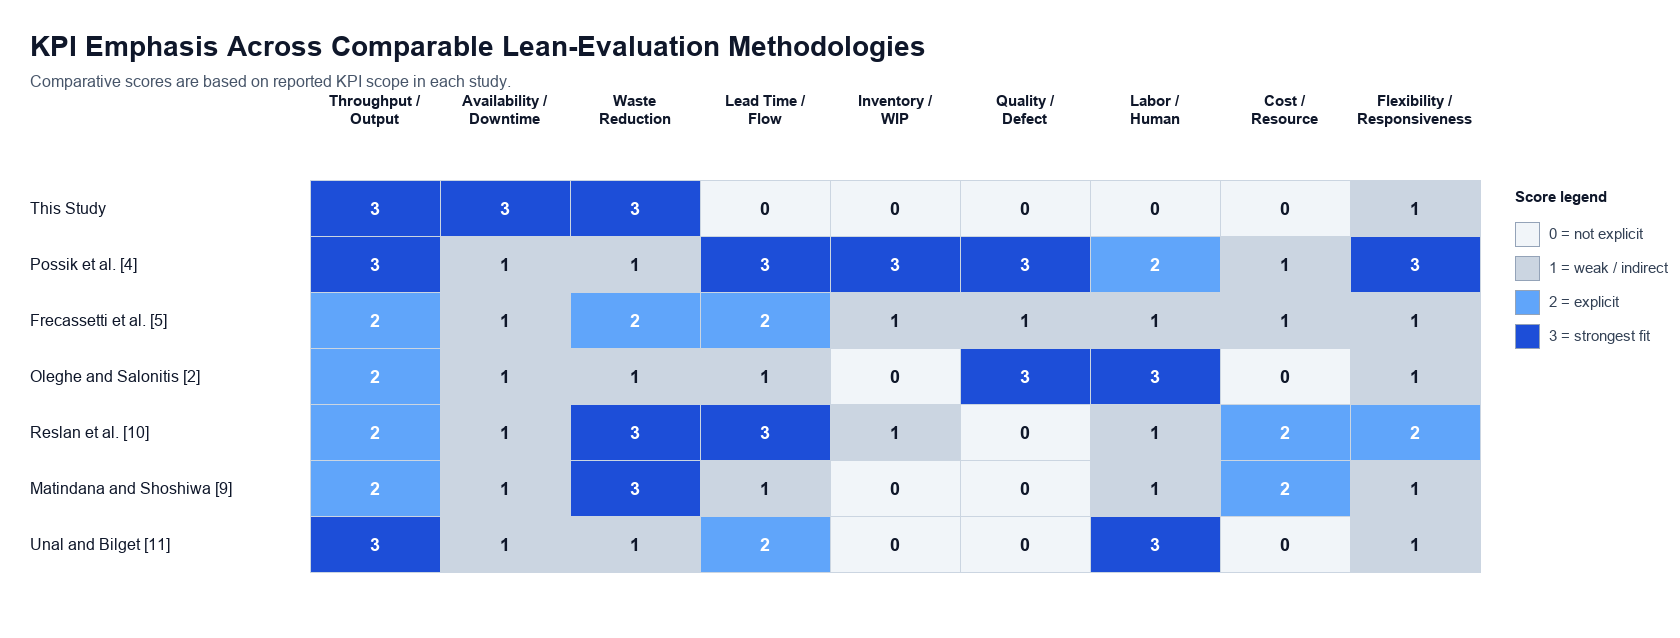
\includegraphics[width=0.98\textwidth]{outputs/methodology_kpi_heatmap.png}
\caption{KPI-based comparison of the proposed methodology with comparable lean-evaluation studies.}
\end{figure}

\begin{figure}[H]
\centering
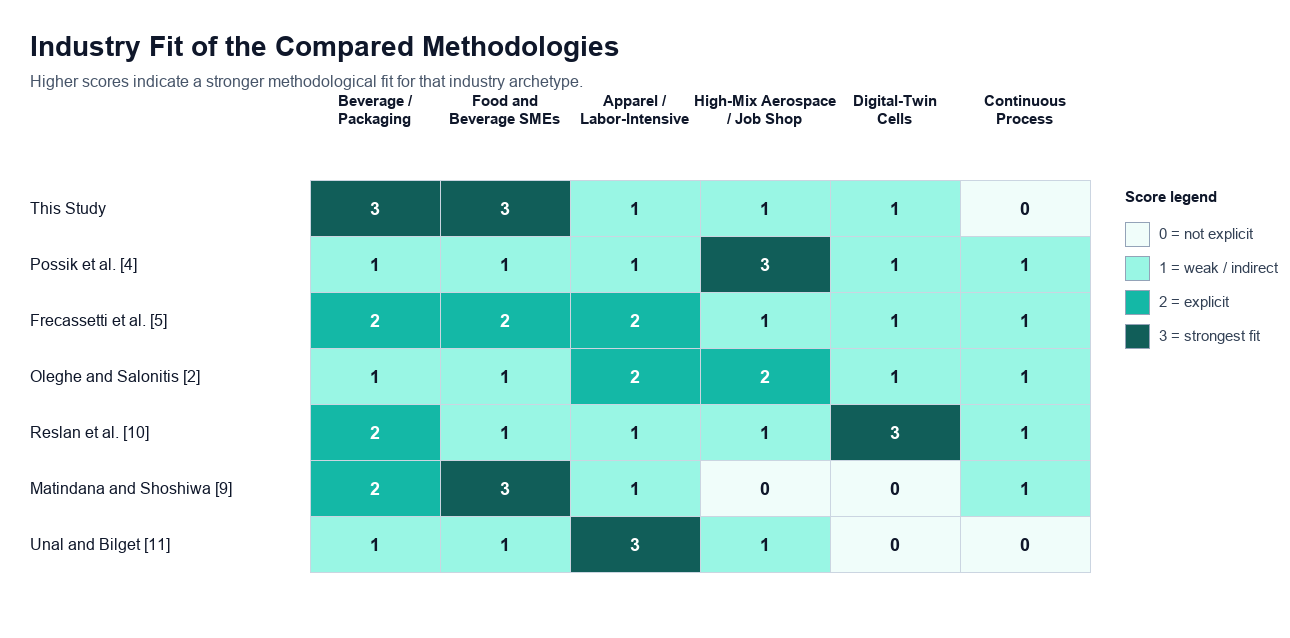
\includegraphics[width=0.98\textwidth]{outputs/methodology_industry_fit_heatmap.png}
\caption{Industry-fit comparison of the scored methodologies.}
\end{figure}

The comparison shows that the present method is powerful in throughput-, downtime-, and waste-reduction-oriented problems. It is suitable for repetitive, machine-paced industries like beverage bottling, food packaging, dairy filling, and similar FMCG-like companies. It is less suitable when the actual decision problem concerns defect generation, labor balancing, WIP, or real-time digital control.

\subsection{Practical Implications}
Based on the results, the priority order of lean implementation is:
\begin{enumerate}
    \item \textbf{First priority: TPM.} TPM should be implemented first, targeting long-duration stoppages through preventive maintenance planning, scheduled tool or equipment checks, fast fault recovery, and reliability tracking.
    \item \textbf{Second priority: 5S and visual management.} Once the regular checkups are established, 5S and visual management should be used to reduce small disruptions, improve operator control, and standardize the workplace.
    \item \textbf{Third priority: integrated lean bundle.} Once maintenance discipline is improved, the plant can combine TPM with micro-stop reduction and standard work for higher output gains.
\end{enumerate}

\begin{table}[H]
\centering
\caption{Recommended Lean Implementation Roadmap}
\begin{tabular}{p{1.3cm}p{2.6cm}p{4.0cm}p{5.2cm}}
\toprule
\textbf{Priority} & \textbf{Lean Focus} & \textbf{Expected Impact} & \textbf{Primary KPIs to Monitor} \\
\midrule
1 & TPM and maintenance discipline & Highest reduction in lost-time severity and waiting waste by targeting major stoppages. & Major-downtime minutes, waiting-waste hours, availability, MTTR, major-stoppage count, liters gained. \\
2 & 5S and visual management & Better workplace organization and reduction in frequent micro-disruptions. & Micro-stoppage count, short-delay frequency, operator recovery time, pause reduction, waste reduction (\%). \\
3 & Integrated lean bundle & Combined gains from reliability, stabilization, and standardized work. & Output gain (\%), availability gain, total pause time, waiting-waste share, OEE when quality data are added. \\
\bottomrule
\end{tabular}
\end{table}

\subsection{Limitations and Future Scope}
This paper has four main limitations. The first one is that the lean structures are simulated and assumed rather than observed after the implementation outcomes. The second one is that the dataset does not have any detailed cause-coded downtime labels, so that mapping from downtime category to lean tool remains implicit. The third one is that the analysis is based on only one industrial case, not many, so the result should not be generalized to all production systems mechanically. The fourth one is that the cross-study analysis scores are explanatory scores derived from published methodology descriptions and key performance index (KPI) scopes rather than normalized one-on-one experiments on the same production dataset.

Future work can improve the present study by collecting root-cause-analysis downtime data, operator-level observations, quality-loss information, and real post-intervention performance records. Future studies may also extend the simulation to include changeover analysis, workforce allocation, line balancing, and cost-benefit evaluation.

\section{Conclusion}
This paper shows how lean-manufacturing priorities should be selected in a beverage bottling line by using real production and downtime data. The analysis showed that the machine is not running most of the time, pause time is high, and performance was not consistent across the monitoring period. In lean terms, the line is dominated by waiting waste, because more than half of monitored time is consumed without producing output. Although micro-stoppages occurred most often, they were not the main source of lost production time.

The simulation results show the following patterns:
\begin{enumerate}
    \item 5S and visual management improve output by 2.33\% and reduce waiting waste by 1.52\%;
    \item TPM improves output by 20.61\% and reduces waiting waste by 14.68\%; and
    \item the integrated lean bundle improves output by 32.19\%, raises simulated availability from 42.37\% to 55.33\%, and reduces waiting waste by 22.51\%.
\end{enumerate}

The result confirms that the greatest improvement comes from resolving the severe stoppages before focusing on the frequent but lower-impact micro-stoppages. For this production line, TPM is the most logical first method, while 5S and visual management become more valuable as support after the major downtime is brought under better control. The same conclusion holds whether the system is judged by throughput, availability, or waste reduction.

This paper also shows that the proposed framework is most appropriate for repetitive, downtime-driven SME production systems such as bottling and packaging lines. Its value lies in linking lean decisions to actual loss behavior observed in the plant and in translating downtime into a measurable waiting-waste outcome. In that sense, the study contributes a practical and reproducible method for selecting lean priorities from real industrial data.

\begin{thebibliography}{33}

\bibitem{r1}
I. Belekoukias, J. A. Garza-Reyes, and V. Kumar, ``The impact of lean methods and tools on the operational performance of manufacturing organisations,'' International Journal of Production Research, vol. 52, no. 18, pp. 5346--5366, 2014, doi: 10.1080/00207543.2014.903348.

\bibitem{r2}
O. Oleghe and K. Salonitis, ``Hybrid simulation modelling of the human-production process interface in lean manufacturing systems,'' International Journal of Lean Six Sigma, vol. 10, no. 2, pp. 665--690, 2019, doi: 10.1108/IJLSS-01-2018-0004.

\bibitem{r3}
F. Yu and Z. Chen, ``Tools, application areas and challenges of factory simulation in Small and Medium-Sized Enterprises -- A Review,'' Procedia CIRP, vol. 104, pp. 399--404, 2021, doi: 10.1016/j.procir.2021.11.067.

\bibitem{r4}
J. Possik, A. Zouggar-Amrani, B. Vallespir, and G. Zacharewicz, ``Lean techniques impact evaluation methodology based on a co-simulation framework for manufacturing systems,'' International Journal of Computer Integrated Manufacturing, vol. 35, no. 1, pp. 91--111, 2022, doi: 10.1080/0951192X.2021.1972468.

\bibitem{r5}
S. Frecassetti, B. Kassem, K. Kundu, M. Ferrazzi, and A. Portioli-Staudacher, ``Introducing Lean practices through simulation: A case study in an Italian SME,'' Quality Management Journal, vol. 30, no. 2, pp. 90--104, 2023, doi: 10.1080/10686967.2023.2171326.

\bibitem{r6}
J. A. C. Bokhorst, W. Knol, J. Slomp, and T. Bortolotti, ``Assessing to what extent smart manufacturing builds on lean principles,'' International Journal of Production Economics, vol. 253, art. no. 108599, 2022, doi: 10.1016/j.ijpe.2022.108599.

\bibitem{r7}
G. A. David, P. M. C. Monson, C. Soares Junior, P. O. Concei\c{c}\~ao Junior, P. R. Aguiar, and A. Simeone, ``IoT-Driven Deep Learning for Enhanced Industrial Production Forecasting,'' IEEE Internet of Things Journal, vol. 11, no. 23, pp. 38486--38495, 2024, doi: 10.1109/JIOT.2024.3447579.

\bibitem{r8}
G. A. David, P. M. C. Monson, and C. Soares Junior, Industrial Production Time-Series Dataset from a Beverage Bottling Line. Zenodo, Jan. 4, 2026. doi: 10.5281/zenodo.18146866.

\bibitem{r9}
J. M. Matindana and M. J. Shoshiwa, ``Lean manufacturing implementation in food and beverage SMEs in Tanzania: using structural equation modelling (SEM),'' Management System Engineering, vol. 4, no. 1, pp. 1--14, 2025, doi: 10.1007/s44176-025-00036-3.

\bibitem{r10}
M. Reslan, M. J. Triebe, R. Venketesh, and A. J. Hartwell, ``Automation of Value Stream Mapping: A Case Study on Enhancing Lean Manufacturing Tools Through Digital Twins,'' Procedia CIRP, vol. 134, pp. 455--460, 2025, doi: 10.1016/j.procir.2025.02.159.

\bibitem{r11}
C. Unal and S. Bilget, ``Examination of lean manufacturing systems by simulation technique in apparel industry,'' The Journal of The Textile Institute, vol. 112, no. 3, pp. 377--387, 2021, doi: 10.1080/00405000.2020.1756104.

\bibitem{r12}
M. M. Shahriar, M. S. Parvez, M. A. Islam, and S. Talapatra, ``Implementation of 5S in a plastic bag manufacturing industry: A case study,'' Cleaner Engineering and Technology, vol. 8, art. no. 100488, 2022, doi: 10.1016/j.clet.2022.100488.

\bibitem{r13}
P. M. Rojasra and M. N. Qureshi, ``Performance Improvement through 5S in Small Scale Industry: A case study,'' International Journal of Modern Engineering Research, vol. 3, no. 3, pp. 1654--1660, 2013.

\bibitem{r14}
C. M. L. Rahman, M. A. Hoque, and S. M. Uddin, ``Assessment of Total Productive Maintenance Implementation through Downtime and Mean Downtime Analysis (Case study: a Semi-automated Manufacturing Company of Bangladesh),'' IOSR Journal of Engineering, vol. 4, no. 9, pp. 38--47, 2014, doi: 10.9790/3021-04943847.

\bibitem{r15}
G. Pinto, F. J. G. Silva, A. Baptista, N. O. Fernandes, R. Casais, and C. Carvalho, ``TPM implementation and maintenance strategic plan -- a case study,'' Procedia Manufacturing, vol. 51, pp. 1423--1430, 2020, doi: 10.1016/j.promfg.2020.10.198.

\bibitem{r16}
R. Shah and P. T. Ward, ``Lean manufacturing: context, practice bundles, and performance,'' Journal of Operations Management, vol. 21, no. 2, pp. 129--149, 2003, doi: 10.1016/S0272-6963(02)00108-0.

\bibitem{r17}
L. W. Friedman and H. H. Friedman, ``Analyzing Simulation Output Using the Bootstrap Method,'' Simulation, vol. 64, no. 2, pp. 95--100, 1995, doi: 10.1177/003754979506400203.

\bibitem{r18}
A. Belhadi, Y. B. M. Sha'ri, F. E. Touriki, and S. El Fezazi, ``Lean production in SMEs: literature review and reflection on future challenges,'' Journal of Industrial and Production Engineering, vol. 35, no. 6, pp. 368--382, 2018, doi: 10.1080/21681015.2018.1508081.

\bibitem{r19}
M. Dora, M. Kumar, D. Van Goubergen, A. Molnar, and X. Gellynck, ``Operational performance and critical success factors of lean manufacturing in European food processing SMEs,'' Trends in Food Science \& Technology, vol. 31, no. 2, pp. 156--164, 2013, doi: 10.1016/j.tifs.2013.03.002.

\bibitem{r20}
T. Al-Hawari, F. Aqlan, M. Al-Buhaisi, and Z. Al-Faqeer, ``Simulation-based analysis and productivity improvement of a fully automatic bottle-filling production system: A practical case study,'' in 2010 International Conference on Computer Modeling and Simulation, vol. 4, pp. 195--199, 2010, doi: 10.1109/ICCMS.2010.212.

\bibitem{r21}
I. Zennaro, D. Battini, F. Sgarbossa, A. Persona, and R. De Marchi, ``Micro downtime: Data collection, analysis and impact on OEE in bottling lines: The San Benedetto case study,'' International Journal of Quality \& Reliability Management, vol. 35, no. 4, pp. 965--995, 2018, doi: 10.1108/IJQRM-11-2016-0202.

\bibitem{r22}
G. K. Inyiama and S. A. Oke, ``Maintenance downtime evaluation in a process bottling plant,'' International Journal of Quality \& Reliability Management, vol. 38, no. 1, pp. 229--248, 2020, doi: 10.1108/IJQRM-12-2018-0340.

\bibitem{r23}
C. Cuggia-Jim\'enez, E. Orozco-Acosta, and D. Mendoza-Galvis, ``Lean manufacturing: a systematic review in the food industry,'' Informaci\'on Tecnol\'ogica, vol. 31, no. 5, pp. 163--172, 2020, doi: 10.4067/S0718-07642020000500163.

\bibitem{r24}
J. P. Womack and D. T. Jones, Lean Thinking: Banish Waste and Create Wealth in Your Corporation. New York, NY, USA: Simon \& Schuster, 1996.

\bibitem{r25}
R. Shah and P. T. Ward, ``Defining and developing measures of lean production,'' Journal of Operations Management, vol. 25, no. 4, pp. 785--805, 2007, doi: 10.1016/j.jom.2007.01.019.

\bibitem{r26}
J. Bhamu and K. S. Sangwan, ``Lean manufacturing: literature review and research issues,'' International Journal of Operations \& Production Management, vol. 34, no. 7, pp. 876--940, 2014, doi: 10.1108/IJOPM-08-2012-0315.

\bibitem{r27}
T. Melton, ``The benefits of lean manufacturing: What lean thinking has to offer the process industries,'' Chemical Engineering Research and Design, vol. 83, no. 6, pp. 662--673, 2005, doi: 10.1205/cherd.04351.

\bibitem{r28}
S. Nakajima, Introduction to TPM: Total Productive Maintenance. Portland, OR, USA: Productivity Press, 1988.

\bibitem{r29}
P. Muchiri and L. Pintelon, ``Performance measurement using overall equipment effectiveness (OEE): literature review and practical application discussion,'' International Journal of Production Research, vol. 46, no. 13, pp. 3517--3535, 2008, doi: 10.1080/00207540601142645.

\bibitem{r30}
B. Dal, P. Tugwell, and R. Greatbanks, ``Overall equipment effectiveness as a measure of operational improvement -- A practical analysis,'' International Journal of Operations \& Production Management, vol. 20, no. 12, pp. 1488--1502, 2000, doi: 10.1108/01443570010355750.

\bibitem{r31}
L. del C. Ng Corrales, M. P. Lamb\'an, M. E. Hernandez Korner, and J. Royo, ``Overall equipment effectiveness: systematic literature review and overview of different approaches,'' Applied Sciences, vol. 10, no. 18, art. no. 6469, 2020, doi: 10.3390/app10186469.

\bibitem{r32}
I. P. S. Ahuja and J. S. Khamba, ``Total productive maintenance: literature review and directions,'' International Journal of Quality \& Reliability Management, vol. 25, no. 7, pp. 709--756, 2008, doi: 10.1108/02656710810890890.

\bibitem{r33}
F. A. Abdulmalek and J. Rajgopal, ``Analyzing the benefits of lean manufacturing and value stream mapping via simulation: A process sector case study,'' International Journal of Production Economics, vol. 107, no. 1, pp. 223--236, 2007, doi: 10.1016/j.ijpe.2006.09.009.

\end{thebibliography}

\end{document}
